% Документ принадлежит классу article
%\documentclass[a5paper,8pt]{article} 

% Документ принадлежит классу article, боковые отступы для двустраничной печати.
 \documentclass[twoside,a5paper,landscape,8pt]{article}

% нормальный юникод и русский язык
\usepackage{cmap}
\usepackage[T2A]{fontenc}
\usepackage[utf8]{inputenc} 
\usepackage[russian,english]{babel} % Пакет поддержки русского языка
% \usepackage[unicode,dvipdfm]{hyperref}
% \usepackage[pdftex,unicode]{hyperref}

% элементы документа
\usepackage{graphicx}
\usepackage{tabularx}
\usepackage{tabulary}
\usepackage{longtable,tabu}

% показывать структуру страницы в виде рамок: поля, отступы и т.п
%\usepackage{showframe}
%\usepackage{fullpage}
\usepackage[margin=15mm]{geometry}

% ширина картинок с изображением деталей
\newlength{\picwidth}
\setlength{\picwidth}{30mm}

% вертикальный отступ между строками таблицы
\renewcommand{\arraystretch}{5}

 \title{Детали набора Робот Машинка, модель 2.1} % Заглавие документа
 \date{\today} % Дата создания

\begin{document}
  \begin{center}
    \textbf{Инструкция по сборке Робота Машинки}\\
    \textbf{подключение проводов}
  \end{center}
  \begin{flushright}
    \emph{модель 2}
  \end{flushright}
   
  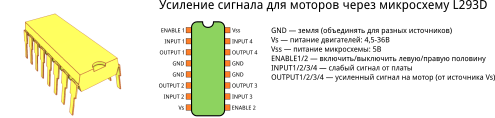
\includegraphics{export/l293d-info.png} \\
  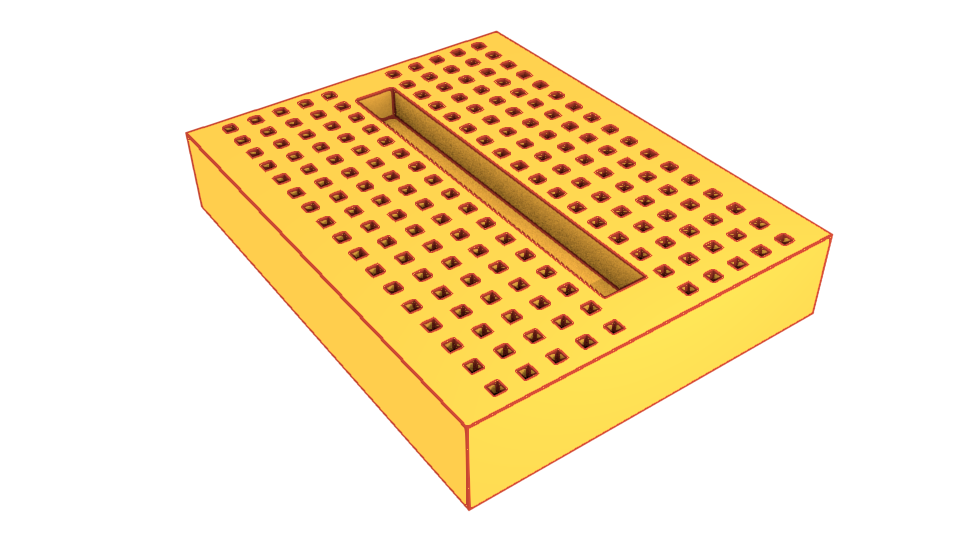
\includegraphics[height=30mm]{export/breadboard-info.png} \\
  
  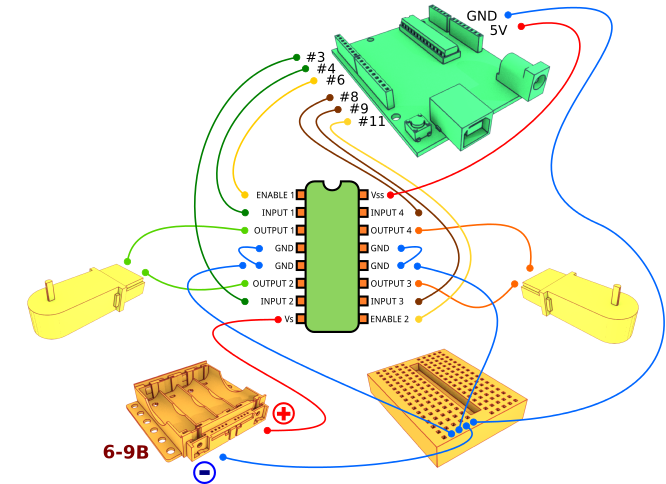
\includegraphics[height=120mm]{export/wiring-final.png}


\end{document}
